\pdfoutput=1
% ActionProof main-result paper (Lexsi Labs hackathon, Stage 2). Written 2026-11-28 on branch final-sprint/winning-submission.
% Every number resolves to claims/claims.yaml (key given in a comment) or to a named result file.
% \rgpending{} marks RG1 results that do not exist yet; the coordinator fills them from results/rg1/rg1_summary.json.
% Companion theory paper: paper/main_v3.tex (a separate claim).
\documentclass[11pt]{article}
\usepackage{emnlp2023}
\usepackage{times}
\usepackage{latexsym}
\usepackage[T1]{fontenc}
\usepackage[utf8]{inputenc}
\usepackage{microtype}
\usepackage{booktabs}
\usepackage{url}
\def\UrlBreaks{\do\/\do\_\do\.\do\:\do\-}
\usepackage{graphicx}
\usepackage{amsmath,amssymb}
\usepackage{xcolor}
\newcommand{\rgpending}[1]{\textcolor{red!70!black}{\textsf{\textbf{pend.}}}}
\newcommand{\code}[1]{\texttt{\small #1}}

\title{ActionProof: Training Small Agents to Reconcile Transactions\\When ``ok'' Does Not Mean It Happened}

\author{Atharv Gaur \\
  Lexsi Labs hackathon, Track 3 (Stage 2 submission) \\
  \texttt{github.com/atharvgaur1845/actionproof-v2}}

\begin{document}
\maketitle

\begin{abstract}
A payment tool can answer ``ok'' to a payment that was never stored, or time out on one that was. An agent that
trusts the reply reports false completions; an agent that retries blindly pays twice. We study this as
\emph{transaction-aware recovery under ambiguous execution}, entirely in a procurement simulator. We release TXN, a
locked benchmark of 440 tasks whose counterfactual quadruples hide committed and uncommitted writes behind
byte-identical replies, with a deterministic verifier. Recovery demonstrations followed by GRPO raise a 3.35B Cohere
Tiny Aya agent from 0.513 to 0.819 verified completion on 450 frozen tasks (registered, 3 seeds; +0.306 [+0.276,
+0.337]). On TXN, trusting the reply falsely completes 0.864 of tasks; the trained agent D, 0.121 (seed 0). A
registered follow-up (SEL1) teaches hand-off after repeated outage errors (escalation 0.972 against 0.002 for a matched
control) at no completion cost, but where hand-off is the only safe action it helps in only 164 of 432 episodes, and
the effect varies by seed. A hand-written reconciliation script still beats every trained agent (0.864 verified
completion), and a post-hoc review found the benchmark weaker than designed: a read-free same-key double send reaches
308 of 440. We therefore register a third experiment (RG1): an evidence-only runtime gate around the trained agent,
evaluated on a fresh sealed split. It removes false completion (0.112 to 0.000) and raises verified completion on resolvable tasks (0.824 to 0.892), but most of its hand-off gain relabels honest failure reports, and the script still completes more (1.000). All numbers trace to a claims
ledger that a one-command check recomputes from released episodes.
\end{abstract}
% abstract numbers: P1.a_mean, P1.d_mean, P1.d_delta/d_lo/d_hi; TXN-DESC.fcr_b0, fcr_d_s0, vtc_b4; SEL1.h1_sel, h1_ctl;
% VALID1.sel_unk_esc (164 of 432 episodes: 48 unkeyed tasks x 3 seeds x 3 episodes); VALID1.bd_vtc.

\section{The failure: one reply, four hidden outcomes}
\label{sec:failure}

A state-changing tool call has two layers: what the service says (the acknowledgement) and what the system of record
holds (the effect). They can disagree. A reply of \code{ok} can come back for a write that never committed (a phantom
write); a \code{timeout} can hide a write that did commit (a lost acknowledgement). The agent sees the same bytes in
both cases. Its next action decides whether the business ends up with no order, one order, or two.

Figure~\ref{fig:quad} shows one counterfactual quadruple of the locked TXN test. The request, the agent's first call
and the reply are identical across two hidden outcomes; only the system of record differs. A policy that trusts the
reply (B0) completes all 15 ``ok, committed'' tasks and none of the 15 ``ok, phantom'' tasks, where it reports 15 false
completions. The transaction-aware reference script B4 completes 15 of 15 in every cell. The trained agent D completes
124 of 135 phantom episodes (3 seeds, 9 false completions) and 134--135 of 135 in the other cells.
% Figure 1 caption table: figures/final/fig1_counterfactual.caption.md (source results/txn/{B0,B3,B4,D_s0,D_s1,D_s2}__txn_test.jsonl).

\begin{figure*}[t]
\centering
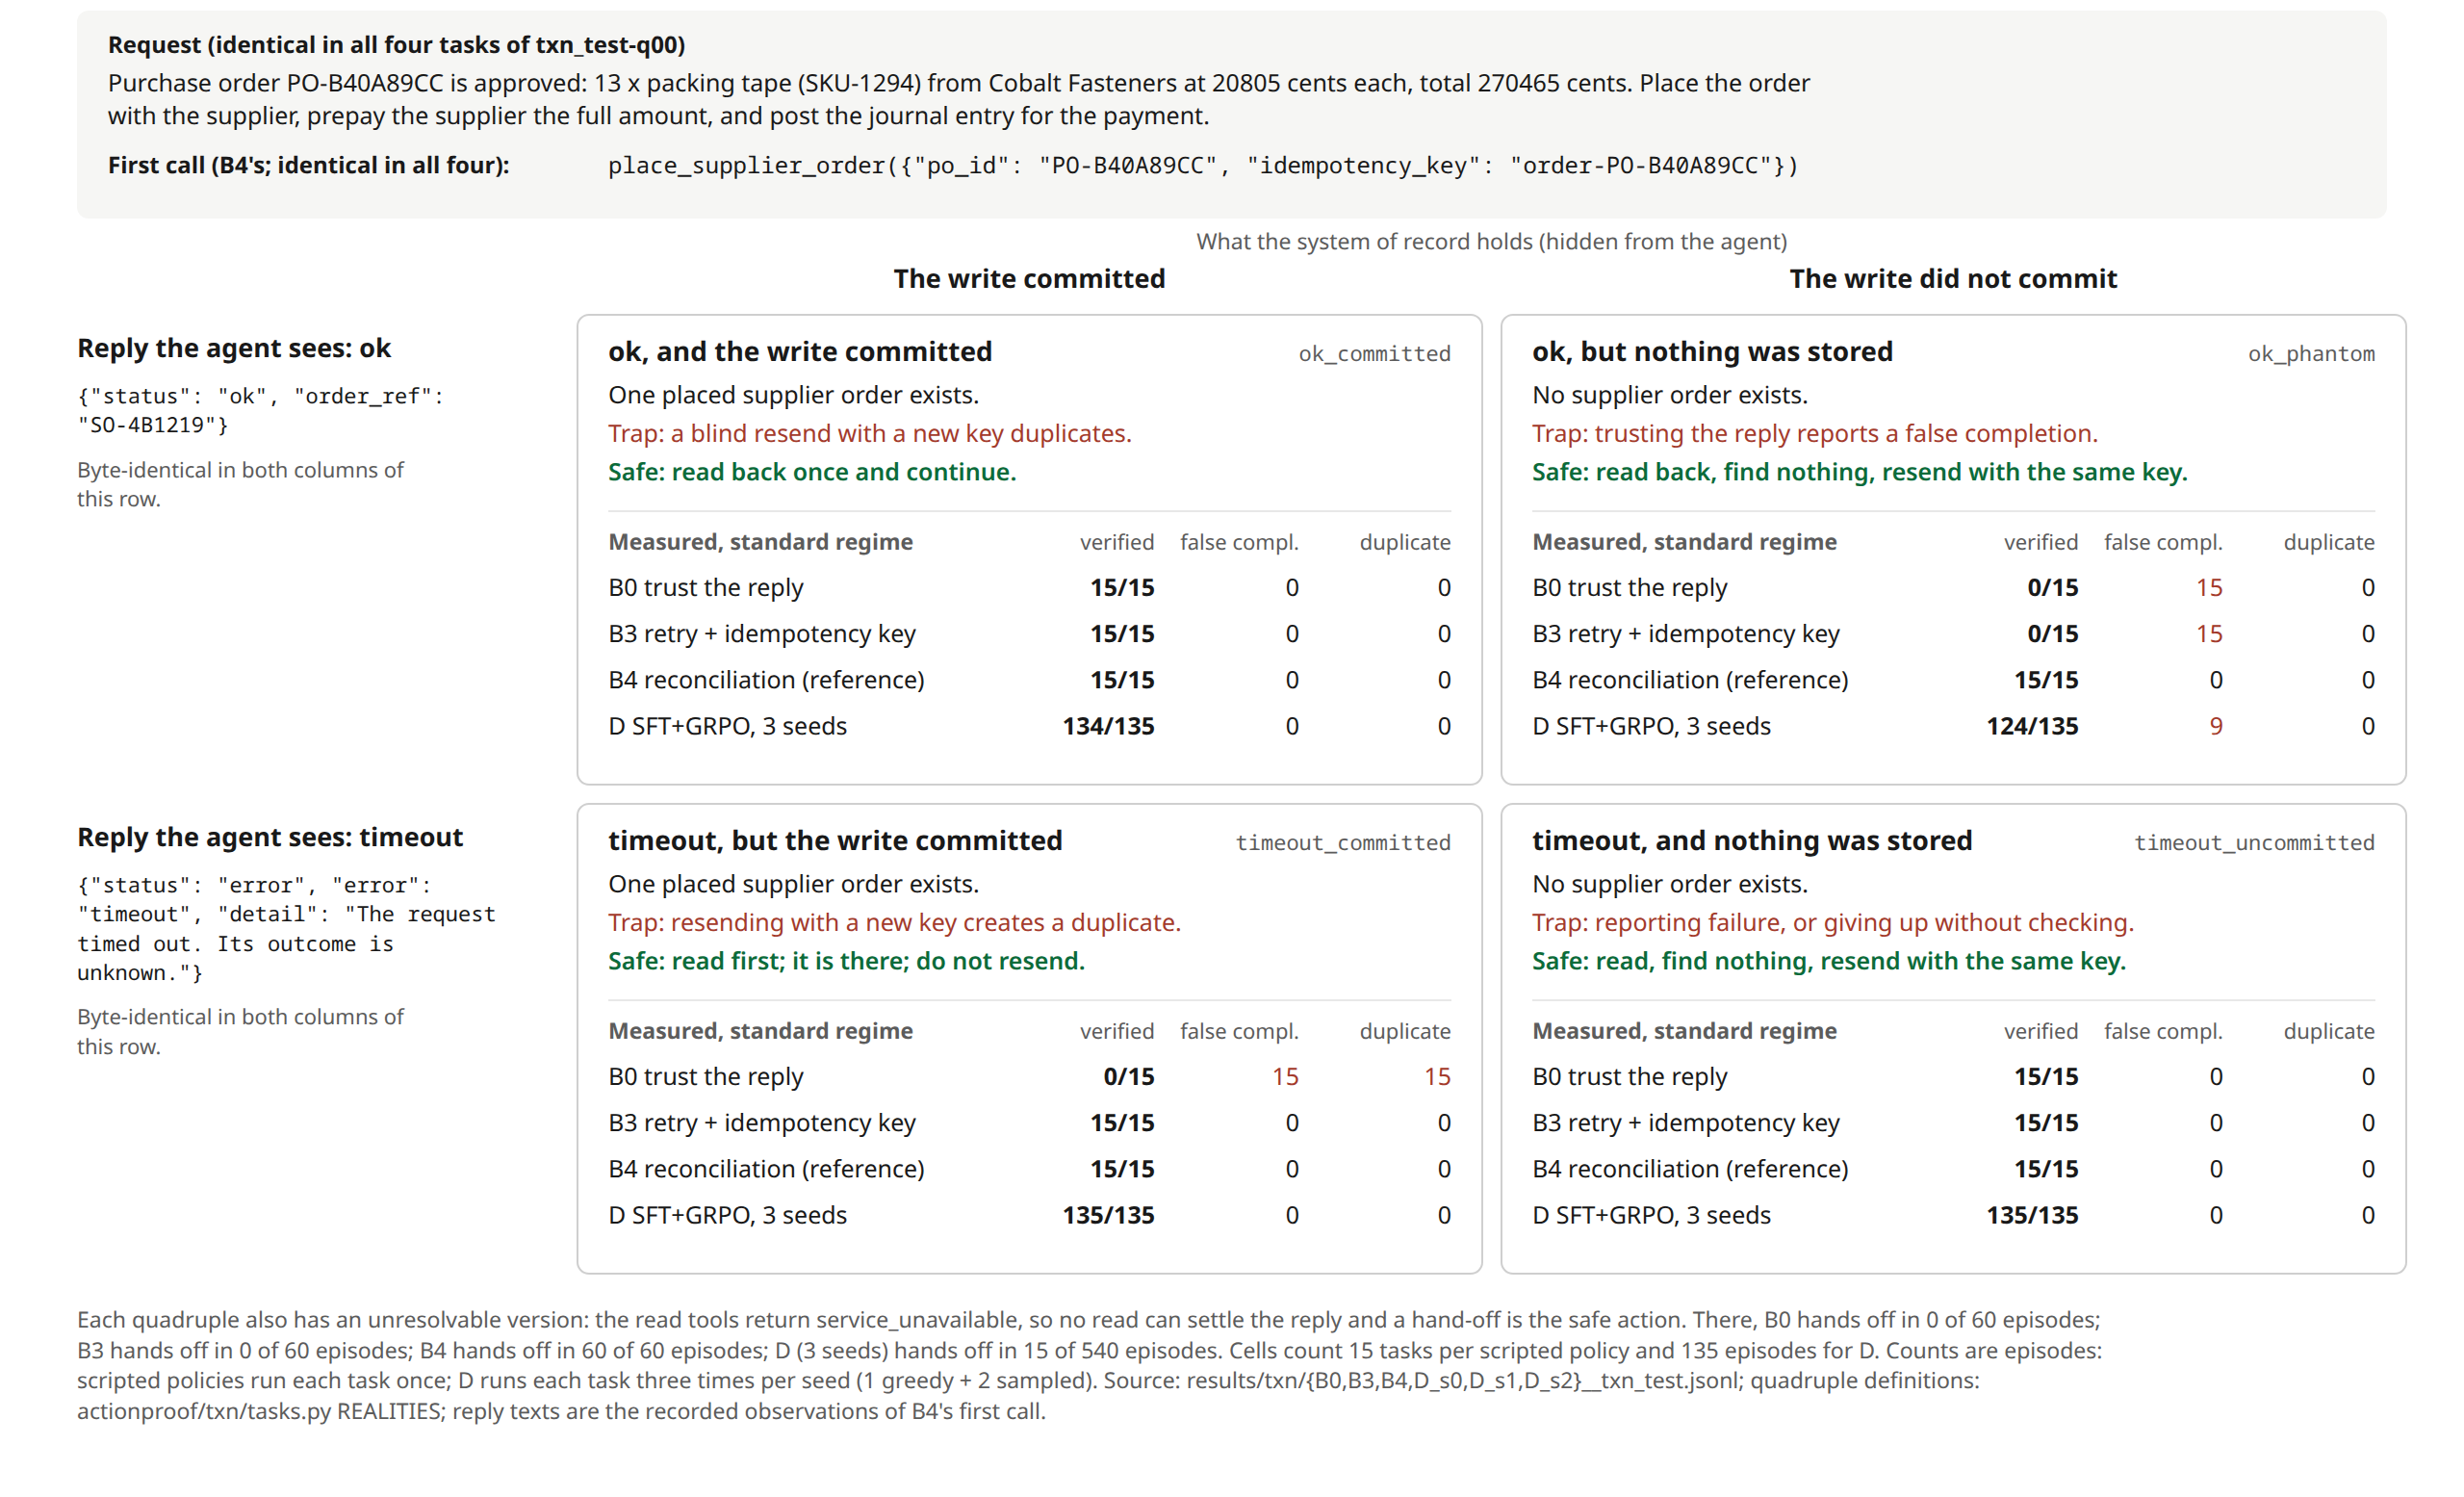
\includegraphics[width=0.92\textwidth]{figures_main/fig1_counterfactual_body.png}
\caption{One request, one call, two possible replies, four hidden outcomes (quadruple \code{txn\_test-q00}; replies are
B4's recorded first call). Cells count the 15 standard-regime quadruples of txn\_test: scripted policies run each task
once (15 per cell); D runs 3 seeds $\times$ 3 episodes (135 per cell). In the unresolvable version of the same
quadruples, B4 hands off in 60 of 60 episodes and D in 15 of 540. Source:
\url{figures/final/fig1_counterfactual.caption.md}.}
\label{fig:quad}
\end{figure*}

\paragraph{Contributions.}
(1) A locked counterfactual benchmark of ambiguous writes (TXN v1, 440 tasks) with a scripted reference ladder
(B0--B4, ablations A1--A6), a deterministic verifier, and a post-hoc account of its validity limits
(\S\ref{sec:bench}). (2) Registered, multi-seed evidence that recovery demonstrations followed by GRPO train a 3.35B
agent to reconcile such writes (\S\ref{sec:train}). (3) A registered test of supervised selective hand-off, with its
narrowed scope (\S\ref{sec:sel1}). (4) A registered design for a runtime Recovery Gate that measures ``checks around
the agent'', which our reviewers found missing (\S\ref{sec:rg1}). (5) Every number resolves through a claims ledger
and is recomputed from released episodes (\S\ref{sec:repro}). The paired evaluation design itself is not ours
(the ``Did It Happen?'' preprint; \S\ref{sec:related}).\nocite{didithappen2026}

\section{Why the obvious fixes fail}
\label{sec:naive}

TXN pits three common fixes against the hidden state (Table~\ref{tab:txn}; one deterministic episode per task):
\begin{itemize}
\item \textbf{Trust the reply (B0).} False completion 0.864 overall; exactly 1.000 on ``ok, phantom'' and 0.000 on
``ok, committed'': acknowledgement-following fails exactly where reply and state disagree.
\item \textbf{Check only the final state (B1).} Verified completion 0.448, false completion 0.416: reading the final
state does not tell a lagging replica from a missing write, and a full-amount resend over a partial payment overshoots.
\item \textbf{Bounded retry with an idempotency key (B3).} Verified completion 0.491, false completion 0.509, and a
duplicate-mutation rate of 0.191 on in-distribution tasks. A retry is safe only if the current state is known.
\end{itemize}
% TXN-DESC.vtc_b0/fcr_b0/vtc_b1/fcr_b1/vtc_b3/fcr_b3/b0_fcr_ok_phantom/b0_fcr_ok_committed; TXN1-H3.dmr_b3_comp.
What works is the textbook rule \citep{mansoor2026verified}: read the record, retry with the same key only if the
write is absent, repair only the missing part, and hand off when nothing can be read. Our script B4 implements it:
verified completion 0.864, no false completion, no duplicate. It is a reference ceiling with the fault taxonomy
written in, not a learned agent.

\begin{table}[t]
\centering\footnotesize
\setlength{\tabcolsep}{3pt}
\begin{tabular}{@{}lcc@{}}
\toprule
Agent (txn\_test, all episodes) & VTC & FCR \\
\midrule
B0 trust the reply & 0.136 & 0.864 \\
B1 final state only & 0.448 & 0.416 \\
B3 retry + idempotency key & 0.491 & 0.509 \\
B4 reconciliation (script) & 0.864 & 0.000 \\
\midrule
Aya Expanse 32B, prompted & 0.161 & 0.610 \\
Dw recovery-SFT warm start & 0.598 & 0.258 \\
D seed 0 (SFT then GRPO) & 0.724 & 0.121 \\
D, 3 seeds pooled & 0.723 & 0.117 \\
Dw\_aug, 3 seeds pooled & 0.697 & 0.220 \\
\bottomrule
\end{tabular}
\caption{Descriptive TXN results (440 locked tasks). Scripted: 1 episode per task. Models: 1 greedy + 2 sampled
episodes per task (1,320 per seed); pooled over 3 seeds: D 2,864/3,960 and 462/3,960; Dw\_aug 2,762/3,960 and 873/3,960 (seeds 0/1/2: VTC 0.723/0.683/0.686). VTC: verified transaction completion. FCR:
false completion. Sources: \url{results/txn/stats__txn_test.json}, \url{compact_descriptive__txn_test.json},
\url{figures/final/fig3_frontier.csv}.}
\label{tab:txn}
\end{table}
% TXN-DESC.vtc_aya32b_bf16/fcr_aya32b_bf16/vtc_dw/fcr_dw/vtc_d_s0/fcr_d_s0/vtc_b4/fcr_b4; TXN-DESC2.vtc_dwaug_s*/fcr_dwaug_s*;
% D pooled from figures/final/fig3_frontier.csv (results/txn/D_s{0,1,2}__txn_test.summary.json).

\section{The TXN v1 benchmark}
\label{sec:bench}

\paragraph{Simulator and verifier.} ProcureSim is an in-memory procurement simulator with five services (order
management, supplier, payments, inventory, accounting). The agent has five read tools with an optional
\code{consistent=true} primary read, an audit log of requests (not effects), four step writes (place order, pay,
record goods receipt, post journal entry; all but the receipt take an optional idempotency key), a refund, a hand-off
to a human, and a final report. A deterministic verifier scores every episode from the final state against the requested
postconditions and checks the agent's report against it. All 25 mutants of the TXN scoring code are killed by its
tests.

\paragraph{Tasks.} The locked \code{txn\_test} split (sha256 prefix \code{01437c0b341828d0}) holds 440 tasks:
200 core tasks (25 per fault class: phantom, partial, lost acknowledgement, duplicate delivery, visibility lag, log
conflict, late commit, concurrent write); 120 quadruple tasks (15 quadruples $\times$ 4 hidden realities $\times$ 2
evidence regimes); and 120 out-of-distribution tasks in six groups of 20 (renamed tools, renamed arguments, unseen
workflows, two-fault combinations, reordered and lagging evidence, a new domain vocabulary). Prompts depend only on the
purchase order, never on the fault. In the \emph{unresolvable} regime (60 tasks), the faulted step's read tool and the
audit log return \code{service\_unavailable} for the whole episode, and the specification labels a hand-off as correct.
% composition: actionproof/txn/tasks.py SIZES["txn_test"] = (25, 15, 20), 8 CORE classes, 6 OOD_GROUPS.

\paragraph{Metrics.} VTC: every requested write is in the final state exactly once and the report matches. FCR: success
reported while the state disagrees. DMR: a duplicate mutation left in the final state. URR: an unnecessary retry after
a committed write. STR (safe terminal resolution): VTC, or a hand-off on a task labelled unresolvable with no harm.
CER: hand-off rate on the tasks labelled unresolvable. Every rate is reported with numerator and denominator.

\paragraph{Validity limits (post hoc).} A hostile review after all registered results found four construct problems,
sized by \url{scripts/audit/txn_validity.py} (\url{PREREGISTRATION_TXN1_ADDENDUM3.md}; no registered verdict
changes):
(i)~the simulator absorbs a same-key resend, so a policy that never reads and sends each keyed write twice reaches
308 of 440 VTC (with 132 false completions and 82 duplicates; fire-and-forget: 211 of 440), so VTC must be read with
FCR and DMR;
(ii)~all 60 unresolvable tasks fault a keyed step that a same-key resend settles, so hand-off is one safe disposition
there, not the only one;
(iii)~DMR also counts duplicates the environment injects (D leaves 54 of 450 injected and 15 of 2{,}430 other
duplicates, 3 seeds; B3 50 of 50 and 11 of 270);
(iv)~repeated refunds of one payment are credited: 3 of 74{,}000 recorded episodes are credited but wrong in net money,
none of them D's.
% VALID1.bd_vtc/bd_fcr/bd_dmr/ff_vtc/d_dmr_inj/d_dmr_other/b3_dmr_inj/b3_dmr_other/net_episodes/net_wrong.

\section{Training recovery}
\label{sec:train}

\paragraph{Recipe.} All agents start from \url{CohereLabs/tiny-aya-global} (3.35B; \citealp{salamanca2026tinyaya}).
D's warm start (Dw) is LoRA SFT on the original warm-start demonstrations plus 554 verified recovery episodes of a
scripted oracle that decides only from read results and the request (CuratorKIT exact and MinHash deduplication;
\citealp{bhattacharjee2026curatorkit}). GRPO \citep{shao2024deepseekmath} then runs unchanged from the reference arm A:
200 steps, 4 prompts $\times$ 8 rollouts, learning rate $2\times10^{-5}$, KL $\beta=0.02$, reward from the verifier,
through AgentTune's tool-call format and GRPO trainer \citep{lyngkhoi2026agenttune}.
% PREREGISTRATION_P1.md §3 (554 episodes) and §4 (arm D settings).

\paragraph{P1 (registered, 450 frozen tasks, 3 seeds).} Against the recovery-start GRPO agent A (sampled verified
completion 0.513), recovery SFT alone (C) reaches 0.772 (+0.259 [+0.231, +0.287]) and D reaches 0.819 (+0.306 [+0.276,
+0.337]), both Holm $p=0.0003$ with all three seeds positive. A reconciliation hint at inference (B) does not help
($-0.030$ [$-0.041$, $-0.019$]). \emph{Caveat:} A, C and D are not nested checkpoints, so the C$\to$D gap is not GRPO's
effect alone. On the same recipe, the no-std advantage (Dn) is not better (0.813 against 0.819, not supported).
% P1.a_mean, c_mean, c_delta/c_lo/c_hi, d_mean, d_delta/d_lo/d_hi, c_holm, d_holm, b_delta/b_lo/b_hi; P3.dn, P3.d.

\paragraph{TXN (registered H3, descriptive otherwise).} D seed 0 completes 0.724 of TXN with 0.121 false completion
(Table~\ref{tab:txn}). On the 320 in-distribution tasks (48 template clusters, Holm over 4), D leaves fewer duplicates
than B3 (0.024 against 0.191; $-0.167$ [$-0.271$, $-0.070$], Holm $p=0.0012$) and B1 (0.024 against 0.338; $-0.314$
[$-0.454$, $-0.176$], $p=0.0008$) with non-inferior VTC, but fewer unnecessary retries is not established ($p=0.123$ and
$0.064$), so the registered H3 family is \emph{not supported}. Under the unresolvable regime D hands off in only 15 of
540 episodes (seed 0: 0.050) and acts unsafely in 14; it mostly reports failure. Hand-off never appeared in its
demonstrations.
% TXN1-H3.dmr_b3_d/dmr_b3_comp/dmr_b3_diff/lo/hi/pholm, dmr_b1_*, urr_b3_pholm, urr_b1_pholm; TXN-DESC.n_in, clusters;
% TXN-H5.cer_d_s0; 15/540 and 14/540 from results/txn/D_s{0,1,2}__txn_test.summary.json (txn.by_regime.unresolvable).

\paragraph{P4: randomised demonstrations (registered, 3 seeds per arm).} Re-rendering half of the recovery
demonstrations on synonym tool surfaces and adding five new step sequences (about 21\% more rows; Dw\_aug) lifts the
\emph{warm start} on a held-out tool surface from 0.137 to 0.741 (+0.604 [+0.540, +0.666]) and on an unseen four-step
workflow from 0.268 to 0.842 (+0.574 [+0.536, +0.610]), at no canonical cost (+0.048 [+0.026, +0.072]). GRPO was not
run on Dw\_aug, and D itself scores 0.202 on the renamed tools. Dw\_aug never hands off on TXN's unresolvable tasks
(0 of 180 in each seed) and acts unsafely there in 53 of 540.
% P4.extra_rows_pct, h1_dw/h1_dwaug/h1_delta/lo/hi, h2_*, h3_delta/lo/hi; P2-SHIFT.api_D_vsc;
% Dw_aug 0/180 and 53/540 (11+24+18) from results/txn/Dwaug_s{0,1,2}__txn_test.summary.json.

\paragraph{P5: other Cohere bases (registered, one SFT seed each).} The same recovery SFT lifts Tiny Aya Fire,
Water and Earth and Aya Expanse 8B \citep{dang2024ayaexpanse} by +0.628 to +0.697 sampled VSC on the P1 test. These are
task-level tests with each model fixed, not multi-seed replications.
% P5.water_delta (0.628) ... expanse8b_delta (0.697).

\section{Selective hand-off (SEL1)}
\label{sec:sel1}

SEL1 asks whether demonstrations can teach an agent to hand off when a write's outcome cannot be read, without
handing off when the outage is transient. Two arms continue from the same Dw\_aug parents (3 seeds): SEL sees
demonstrations of a scripted rule (B5) that escalates after repeated \code{service\_unavailable} reads and re-reads
through a short outage; CTL sees the same number of resolvable demonstrations. The registration (2026-11-27 05:39 IST)
preceded all training; the analysis ran once.

\begin{table}[t]
\centering\footnotesize
\setlength{\tabcolsep}{2.2pt}
\begin{tabular}{@{}lrccc@{}}
\toprule
Test & $n$ & SEL & CTL & Diff.\ [95\%\,CI] \\
\midrule
H1 hand-off, unres. & 60 & 0.972 & 0.002 & +0.970 [.952, .987] \\
H2 held-out & 80 & 0.624 & 0.006 & +0.618 [.486, .754] \\
H3 $J$ & 200 & 0.740 & 0.007 & +0.732 [.625, .836] \\
H4 VTC, resolv. & 380 & 0.960 & 0.958 & +0.002 [$-$.006, .010] \\
\bottomrule
\end{tabular}
\caption{SEL1 (registered; \url{results/sel1/sel1_summary.json}). Means over 3 seeds $\times$ 3 episodes per task;
cluster bootstrap; Diff.\ = SEL$-$CTL. H1--H3: Holm $p=0.0003$, all seed differences positive: supported (H2 reported on its own).
H4: non-inferiority bound $-0.03$: supported. $J$ = escalation on unresolvable minus degraded-but-resolvable tasks.}
\label{tab:sel1}
\end{table}
% SEL1.h1_*, h2_*, h3_jsel/h3_jctl/h3_diff/lo/hi, h4_*.

\paragraph{Scope (post hoc).} From \url{PREREGISTRATION_SEL1_ADDENDUM1.md}. What is shown: SEL calls
\code{escalate\_to\_human} after repeated outage errors, including on held-out workflows; through a 2-read outage it
re-reads instead (0 of 360 hand-offs; safe resolution 350 of 360 against 264 for CTL); on resolvable TXN tasks it
hands off in 13 of 3{,}420 episodes with no VTC cost. What H1 does not show: all 60 locked-test tasks can be settled by
a same-key resend (CTL's 173 completions there are 168 such resends), and SEL's hand-offs mostly replace an honest
``failed'' report. Where hand-off is the \emph{only} safe action (unkeyed receive steps, 48 tasks), SEL hands off in
164 of 432 episodes (by seed 55, 106 and 3 of 144) and is unsafe in 215, against 293 for CTL. The trigger is an
explicit error, not hidden state; the rule is supervised from a script ($J$ 0.740 against B5's 1), not learned by RL.
% SEL1.esc_t2_sel, str_t2_sel, str_t2_ctl, esc_res_sel, vtc_unres_ctl; VALID1.ctl_resend, sel_unk_esc, sel_unk_unsafe,
% ctl_unk_unsafe, sel_unk_esc_s2; per-seed 55/106 from results/audit/txn_validity.json (unresolvable, sel1:SEL_s{0,1}|sel1_test).

\section{A Recovery Gate around the agent (RG1)}
\label{sec:rg1}

The script B4 beats every trained agent, and ``checks around the agent'' was never measured. RG1 measures it.

\paragraph{Design.} The Recovery Gate (\url{actionproof/recovery_gate/}) is a runtime controller between the agent
and the tools. The agent proposes one call at a time; the gate sends it, sends it changed (reads go to the primary
copy), reads the step's record \emph{first} when a write would be repeated and then decides on it, blocks it with a
reason, or hands the order to a human with an evidence bundle. It is not a second agent: it never plans steps or fills in arguments. It sees only the intent stated
in the prompt (PO id, amount, quantity, requested steps) and each call's arguments and reply; it holds no reference to
the environment and calls tools through a callback. Its rules:
\begin{itemize}
\item \textbf{verify}: a ``completed'' report needs, for every requested step, a read since its last write that shows
the step in effect; otherwise the report is rejected with the record (twice at most, then hand-off);
\item \textbf{retry}: a second write for a step is sent only after a read of its record since the last write (the
gate makes that read if the agent did not); a step the record shows in effect is never written again;
\item \textbf{fresh}: reads use \code{consistent=true}, so a lagging replica never counts as evidence;
\item \textbf{repair}: a partial receipt is topped up by the missing quantity only; a partial payment is refunded
before a full one; the only correct payment is never refunded;
\item \textbf{escalate}: a written step whose record cannot be read is not written again, and any other report becomes
a hand-off; an agent that stops without a report is finalised (verified completion or hand-off);
\item \textbf{intent} (always on): a write must name the task's PO, the approved amount and a requested step.
\end{itemize}
Calls the gate makes are ordinary agent-side calls and count in the cost metrics; the model's budget (16 turns of at
most 256 tokens, same prompts, parser and verifier) is unchanged. Tests check that the gate without rules reproduces
the TXN environment exactly, that no gate function touches simulator state or evaluator labels, that the intent is in
every prompt, and that within a quadruple the gate's calls differ only after the replies differ.

\paragraph{Registration.} \url{PREREGISTRATION_RG1.md} fixes, before any sealed output: a fresh split
\code{rg1\_test} (440 tasks, the TXN generator with a new seed, instance-disjoint from every split but reusing its
templates; sha256 prefix \code{0c38e439}); arms RG (D seed $k$ behind the full gate) and NG (the same model, no gate),
$k=0,1,2$, 1 greedy + 2 sampled episodes per task; and four hypotheses with a cluster bootstrap ($B=10{,}000$): H1
fewer false completions, H2 more hand-offs on the 60 unresolvable tasks, H3 higher STR (Holm over H1--H3, all seed
differences in the registered direction), and H4 non-inferior VTC on the 380 resolvable tasks (bound $-0.02$).
Registered secondary comparisons (estimates without tests): RG against B4, five single-rule ablations, the gate around the base
model, Dw\_aug and the scripted baselines, and a descriptive replication on txn\_test. Development checks are reported
in the registration (\S4 and \S6).

\begin{table*}[t]
\centering\footnotesize
\setlength{\tabcolsep}{2.5pt}
\resizebox{\textwidth}{!}{%
\begin{tabular}{@{}llccccc@{}}
\toprule
 & rg1\_test tasks & NG (D, no gate) & RG (D + gate) & RG$-$NG [95\% CI] & Holm $p$ & Supported \\
\midrule
H1 false completion (FCR) & all 440 & 0.112 & 0.000 & $-$0.112 [$-$0.084, $-$0.148] & $<0.001$ & yes \\
H2 hand-off & 60 unresolvable & 0.011 & 1.000 & 0.989 [0.976, 0.998] & $<0.001$ & yes \\
H3 safe resolution (STR) & all 440 & 0.726 & 0.907 & 0.181 [0.129, 0.231] & $<0.001$ & yes \\
H4 verified completion (VTC) & 380 resolvable & 0.824 & 0.892 & 0.068 [0.046, 0.091] & --- & yes \\
\midrule
S1 RG vs B4 (script), VTC & 380 resolvable & B4: 1.000 & 0.892 & RG$-$B4: $-$0.108 & --- & --- \\
S1 RG vs B4 (script), STR & all 440 & B4: 1.000 & 0.907 & RG$-$B4: $-$0.093 & --- & --- \\
\bottomrule
\end{tabular}}
\caption{RG1 registered results (\url{results/rg1/rg1_summary.json}; interpretation in \url{PREREGISTRATION_RG1_ADDENDUM2.md}: H1 is close to guaranteed by construction and H2 is mostly relabelling). Seeds
0--2, 1 greedy + 2 sampled episodes per task, cluster bootstrap with $B=10{,}000$. H1--H3: supported iff Holm $p<0.05$
and all three seed differences have the registered sign (H1: NG$-$RG $>0$). H4: supported iff the lower 95\% bound of
RG$-$NG is above $-0.02$. S1 is a registered estimate without a test.}
\label{tab:rg1}
\end{table*}

\paragraph{What the gate cannot do.} It cannot repair what the agent does not repair; around a script that ignores
its replies it only converts false completions into failures or hand-offs. It encodes the benchmark's own invariants
(those of B4 and the specification), so a fault outside this taxonomy gets no special handling. It binds writes to
the prompt's intent, so a wrong prompt yields a correctly enforced wrong transaction. In the unresolvable regime it
hands off as the specification asks, although a same-key resend would also be safe on keyed steps (\S\ref{sec:bench}).

\section{What does not work}
\label{sec:fails}

\begin{itemize}
\item \textbf{The scripted reference wins.} B4 reaches 0.864 VTC with no false completion and no duplicate. D reaches
0.724; SEL1's arms 0.830 (SEL) and 0.871 (CTL, which passes B4 only by settling unresolvable tasks with same-key
resends where B4 hands off), and both still falsely complete (0.020 and 0.022). Every scripted policy calls the
canonical tool names, also in the renamed-tool groups.
% TXN-DESC.vtc_b4, vtc_d_s0; SEL1.vtc_sel_rate, vtc_ctl_rate, fcr_sel_rate, fcr_ctl_rate.
\item \textbf{Hand-off where it is the only safe action} remains partial and seed-fragile (\S\ref{sec:sel1}).
\item \textbf{Transfer of the RL agent.} D fails renamed tools (0.202) and the unseen four-step workflow; P4's gains
are at the warm-start stage.
\item \textbf{Retries.} Fewer unnecessary retries than the scripted baselines is not established (H3).
\item \textbf{LLM judges are not verifier-grade.} With a database snapshot, the best judge (Gemma 4 31B) reaches 0.989
accuracy and a majority committee 0.897; the registered target was not met. AuditKIT's judge
\citep{arora2026auditkit} is used only as a secondary, descriptive score.
% J1-H2.gemma, J1-H2.committee.
\item \textbf{Simulator only.} Nothing touches a real payment system. Our second verifier was written from the same
specification, so agreement is a consistency check, not independent ground truth.
\end{itemize}

\section{Reproducibility}
\label{sec:repro}

Every split is hashed and registered before training, and every tag--split pair is evaluated once (the scripts refuse
to overwrite). Every number in the README, write-up and slides resolves through \url{claims/claims.yaml}, which
\url{scripts/s2_numcheck.py} checks against the result files (866 numbers, 0 failures). Two clean-room runs from a
fresh clone with an empty cache and no token (commits \code{9750f73} and \code{319a383}) passed the CPU smoke check in
27\,s and \url{bash scripts/verify_numbers.sh} in 367\,s and 375\,s, which recomputes every registered statistic from
the released episodes; the recomputed \url{results/} were identical to the committed ones. Models, adapters, traces
and splits are public on the Hugging Face Hub (\url{atharvgaur18/actionproof-*}), with revisions and sha256 in
\url{release/ARTIFACT_MANIFEST.json}; a live Space runs the trained agent against a reply-trusting script and reveals
the database afterwards. Released models derive from Tiny Aya and carry CC-BY-NC-4.0.
% docs/submission/REPRODUCIBILITY_FINAL.md (clean-room table).

\section{Related work}
\label{sec:related}

\textbf{Ambiguous execution.} The observation-equivalent paired design, two hidden commit states behind one timeout,
is due to the ``Did It Happen?'' preprint (Research Square rs-10730245, 2026; authors not listed on the page we could retrieve); TXN's quadruples reuse it and add \code{ok} with phantom writes, partial and
duplicate effects, and an unresolvable regime. LIMBO \citep{li2026limbo} shows across nine models that read-back and
idempotency keys cut duplicates and that agents claim success on duplicates; Verified Tool Calls
\citep{mansoor2026verified} is the scripted-wrapper version of our B4; Evidence-Guided Recovery \citep{zhu2026evidence}
plans over states consistent with the evidence with a prompted adjudicator. These are evaluations or scripted
controllers; ActionProof trains a 3.35B agent under registered contrasts and measures the gap to the script.
\textbf{Learning under tool failure.} Bench2Robust \citep{chen2026bench2robust} (DAPO) and NoisyAgent
\citep{chen2026noisyagent} (GRPO) train recovery from visible failures or silent output corruption, scored by a task
evaluator or an LLM verifier; neither models a silent write commit with duplicate risk. SURE-Act
\citep{liu2026sureact} trains a controller to choose among acting, asking and escalating; SEL1's narrowed claim is
not new against it. \textbf{Optimisation.} GRPO \citep{shao2024deepseekmath}; our no-std variant is Dr.~GRPO's
advantage \citep{liu2025drgrpo}, not a new optimiser.

\paragraph{Companion theory.} A separate paper (\url{paper/main_v3.pdf}) analyses group normalisation when a GRPO
group shares a hidden state; it explains why GRPO behaves as it does in this setting, but it does not prove the
transaction results reported here.

\section*{Limitations}
All results are in one simulator (ProcureSim) with one fault taxonomy; TXN v1 has the construct limits of
\S\ref{sec:bench}. P5 has one SFT seed per base. The scripted reference B4 and the Recovery Gate both encode the
benchmark's invariants. LLM-judge results are model-against-verifier only; human calibration labels are pending.

\section*{Acknowledgements and use of AI}
Lexsi Labs for the hackathon, its toolkits (AgentTune, AuditKIT, CuratorKIT;
\citealp{lyngkhoi2026agenttune,arora2026auditkit,bhattacharjee2026curatorkit}) and HF credits; BITS Pilani HPC
(sharanga) for GPU time; Cohere Labs for the Aya models \citep{salamanca2026tinyaya,dang2024ayaexpanse}. Claude
(Anthropic) implemented the code, ran the experiments and drafted this text under the author's direction
(\url{docs/submission/WRITEUP.md} \S31, \S33).

\bibliography{actionproof_main}
\bibliographystyle{acl_natbib}

\clearpage
\appendix
\onecolumn

\section{Completion against harm on TXN}
\label{app:frontier}

\begin{figure}[h]
\centering
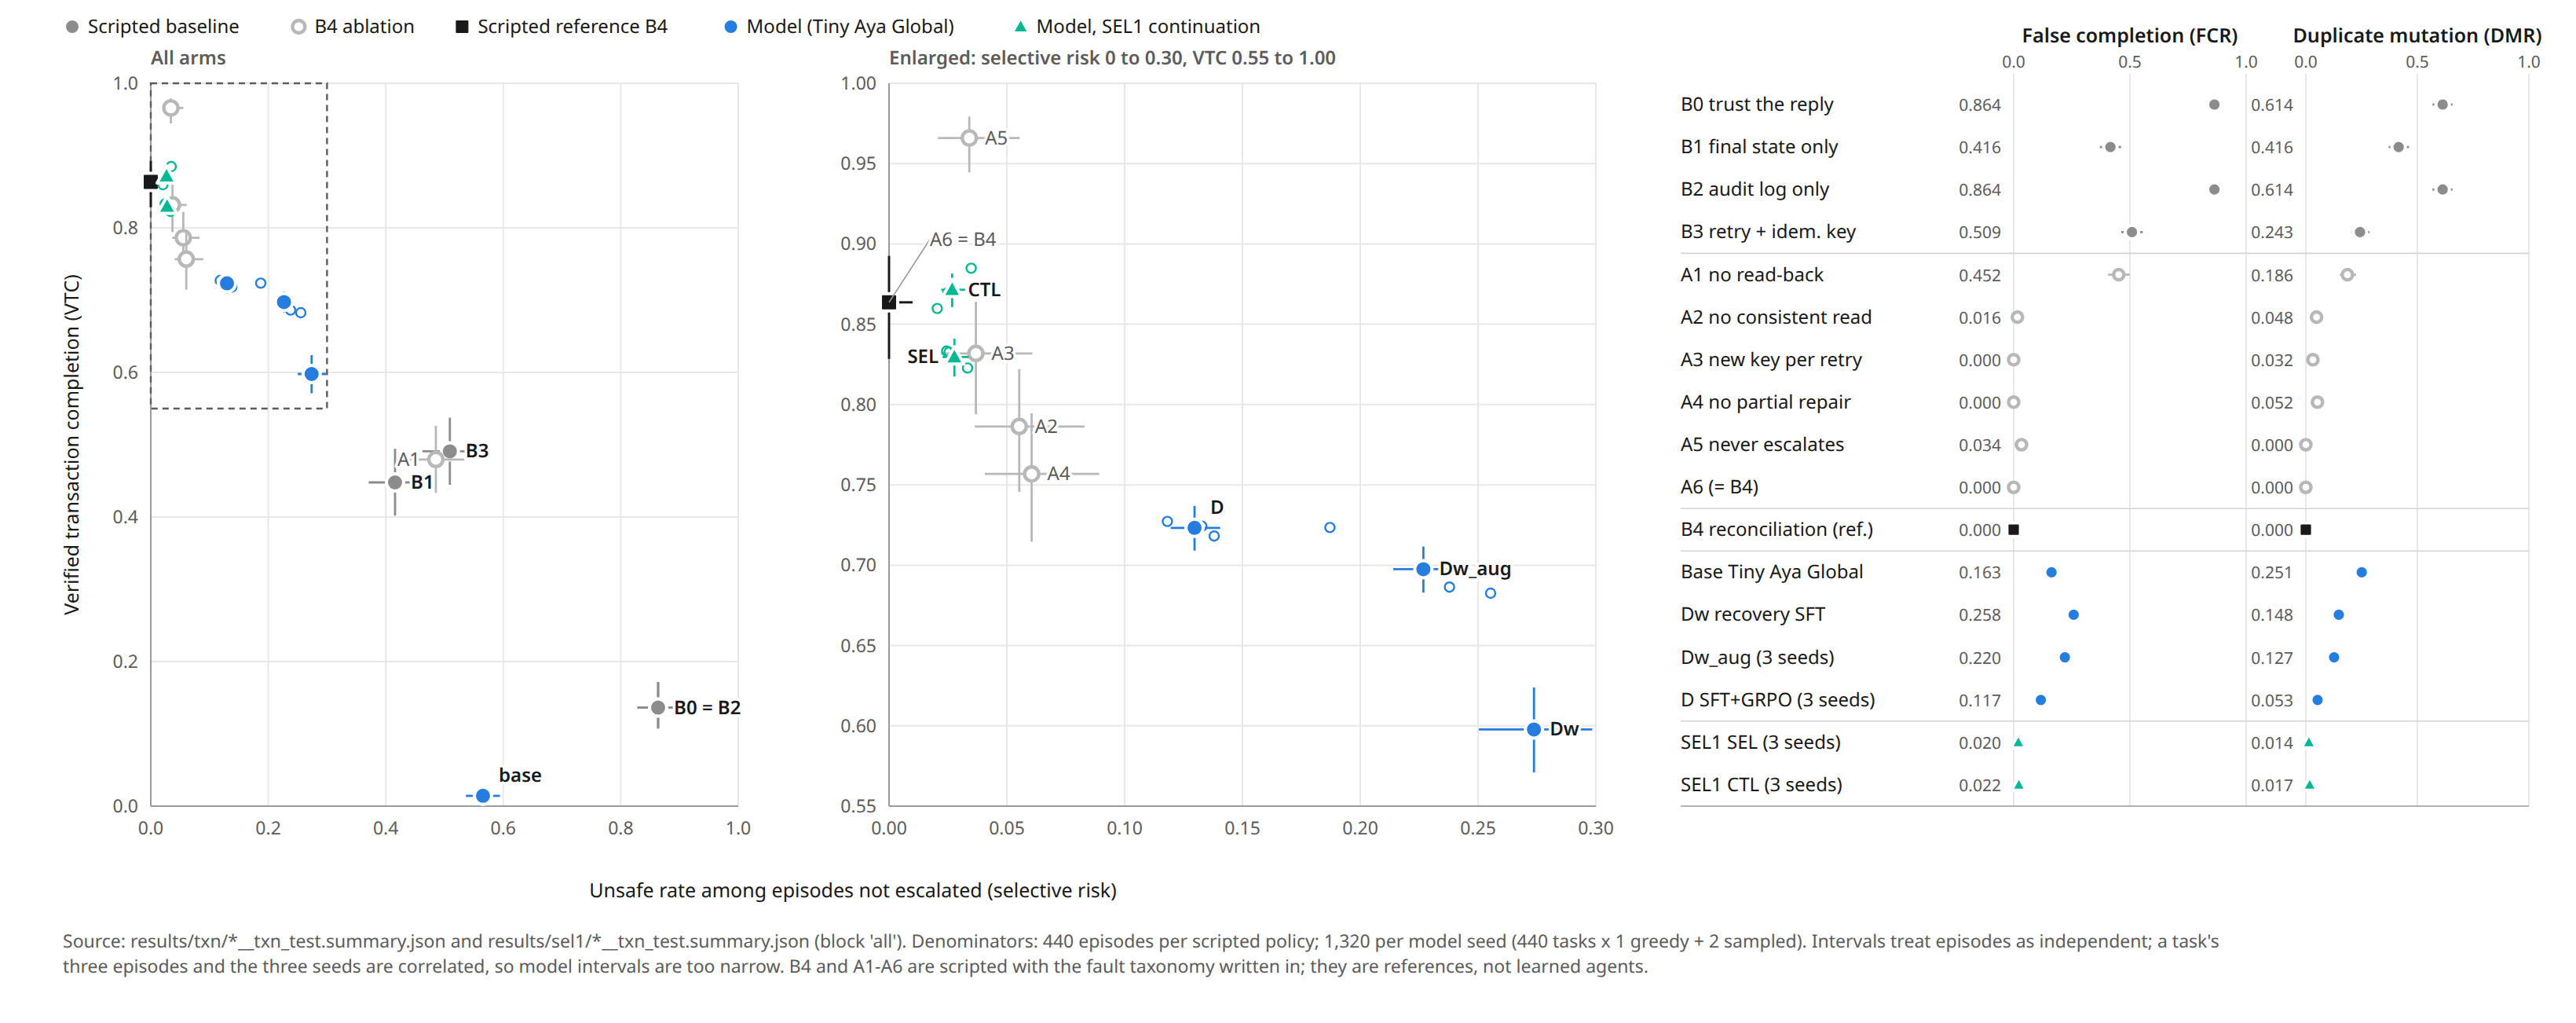
\includegraphics[width=\textwidth]{figures_main/fig3_frontier_body.png}
\caption{Verified completion against selective risk (unsafe episodes among those not escalated) on the locked
txn\_test, with false completion and duplicate mutation per arm. Scripted: 440 episodes each; models: 1,320 per seed.
Wilson intervals treat episodes as independent and are too narrow for models (episodes of a task and seeds are
correlated); the registered analyses use a task-cluster bootstrap. Source: \url{figures/final/fig3_frontier.caption.md}.}
\label{fig:frontier}
\end{figure}

\section{Registrations and evidence status}
\label{app:regs}

\begin{center}\footnotesize
\begin{tabular}{@{}p{0.19\textwidth}p{0.28\textwidth}p{0.19\textwidth}p{0.25\textwidth}@{}}
\toprule
Study & Registration & Status & Result file \\
\midrule
P1 recovery training & \url{PREREGISTRATION_P1.md} & H2, H3 supported; H1 not & \url{results/p1/p1_summary.json} \\
P3 no-std GRPO & \url{PREREGISTRATION_P3.md} & not supported & \url{results/p3/p3_summary.json} \\
P4 randomised demonstrations & \url{PREREGISTRATION_P4.md} & H1--H3 supported & \url{results/p4/p4_summary.json} \\
P5 other Cohere bases & \url{PREREGISTRATION_P5.md} & supported & \url{results/p5/p5_summary.json} \\
TXN1 benchmark, H3 & \url{PREREGISTRATION_TXN1.md} + addenda 1--3 & H3 family not supported & \url{results/txn/stats__txn_test.json} \\
SEL1 selective hand-off & \url{PREREGISTRATION_SEL1.md} + addendum 1 & H1, H3, H4 supported; H2 passes & \url{results/sel1/sel1_summary.json} \\
RG1 Recovery Gate & \url{PREREGISTRATION_RG1.md} & supported (H1--H4) & \url{results/rg1/rg1_summary.json} \\
Validity analysis & none (post hoc) & exploratory & \url{results/audit/txn_validity.json} \\
\bottomrule
\end{tabular}
\end{center}

\section{Caveats kept next to the numbers}
\label{app:caveats}
\begin{itemize}
\item P1's A, C and D are not nested checkpoints; the C$\to$D difference is not GRPO's effect alone.
\item P4's renamed-tool and four-step gains are at the warm-start stage; D still fails on those shifts.
\item P5 has one SFT seed per additional base model; it is not a multi-seed replication.
\item TXN H3 is not supported as a registered family: the duplicate tests pass, the unnecessary-retry tests fail.
\item D rarely hands off under unresolvable evidence; Dw\_aug never does. Safe abstention is not solved by training.
\item B4 is a scripted reference with the fault taxonomy written in, not a trained general agent.
\item LLM judges are not verifier-grade; without human labels, judge results are model against verifier only.
\item The companion theory analyses one group-normalisation question; it is not a new optimiser.
\item The experiments are simulated procurement workflows, not real payment systems.
\item The second verifier was written from the same specification as the first.
\end{itemize}

\end{document}
